\chapter{Results}
\label{chapter:results}
In this chapter we will look at the results of the experiments discussed in chapter~\ref{chapter:experiments}.

\Crefrange{tab:d1}{tab:d4} show the ratio of articles which resulted in no new words, no new pairs or both. In the cases where filtering was applied a shorthand for the filter type (cf=collection frequency, tf=term frequency) is included as well as the threshold. We note that filtering does in fact increase the number of empty output-sets of either size and in the case of the collection frequency and term frequency filters as well as any pre-filtering (Configuration5) the change is quite drastic.

\begin{center}
\begin{table}
  \begin{tabular}{|l|c|c|c|}
    \hline
    &  No new words & No new Pairs & Both (empty enumeration) \\ \hline
    Configuration1                    & 0.04  & 0.03  & 0.01 \\ \hline
    Configuration3 (cf: 5)            & 0.00  & 1.00  & 0.93 \\ \hline
    Configuration3 (tf: 5)            & 0.58  & 0.42  & 0.41 \\ \hline
    Configuration3 (tfidf: 5)         & 0.05  & 0.35  & 0.01 \\ \hline
    Configuration5 (cf: 5)            & 0.19  & 0.92  & 0.85 \\ \hline
    Configuration5 (tf: 5)            & 0.01  & 0.99  & 0.96 \\ \hline
    Configuration5 (tfidf: 5)         & 0.00  & 0.74  & 0.01 \\ \hline
    Configuration6                    & 0.04  & 0.03  & 0.01 \\ \hline
    Configuration6 (tfidf: 5)         & 0.04  & 0.52  & 0.02 \\ \hline
  \end{tabular}
  \caption{The outcomes from running different configurations on dataset D1}
  \label{tab:d1}
\end{table}
\end{center}

\begin{center}
\begin{table}
  \begin{tabular}{|l|c|c|c|}
    \hline
    &  No new words & No new Pairs & Both (empty enumeration) \\ \hline
    Configuration1                    & 0.10  & 0.01  & 0.00 \\ \hline
    Configuration3 (tfidf: 5)         & 0.12  & 0.25  & 0.00 \\ \hline
    Configuration5 (tfidf: 5)         & 0.01  & 0.69  & 0.00 \\ \hline
    Configuration6                    & 0.10  & 0.01  & 0.00 \\ \hline
    Configuration6 (tfidf: 5)         & 0.11  & 0.36  & 0.01 \\ \hline
  \end{tabular}
  \caption{The outcomes from running different configurations on dataset D2}
  \label{tab:d2}
\end{table}
\end{center}

\begin{center}
\begin{table}
  \begin{tabular}{|l|c|c|c|}
    \hline
    &  No new words & No new Pairs & Both (empty enumeration) \\ \hline
    Configuration1                    & 0.16  & 0.10  & 0.01 \\ \hline
    Configuration3 (tfidf: 5)         & 0.16  & 0.30  & 0.01 \\ \hline
    Configuration5 (tfidf: 5)         & 0.11  & 0.55  & 0.01 \\ \hline
    Configuration6                    & 0.16  & 0.10  & 0.01 \\ \hline
    Configuration6 (tfidf: 5)         & 0.16  & 0.32  & 0.01 \\ \hline
  \end{tabular}
  \caption{The outcomes from running different configurations on dataset D3}
  \label{tab:d3}
\end{table}
\end{center}

\begin{center}
\begin{table}
  \begin{tabular}{|l|c|c|c|}
    \hline
    &  No new words & No new Pairs & Both (empty enumeration) \\ \hline
    Configuration1                    & 0.13  & 0.74  & 0.13 \\ \hline
    Configuration3 (tfidf: 5)         & 0.23  & 0.74  & 0.65 \\ \hline
    Configuration5 (tfidf: 5)         & 0.18  & 0.65  & 0.33 \\ \hline
    Configuration6                    & 0.18  & 0.64  & 0.08 \\ \hline
    Configuration6 (tfidf: 5)         & 0.32  & 0.64  & 0.55 \\ \hline
  \end{tabular}
  \caption{The outcomes from running different configurations on dataset D4}
  \label{tab:d4}
\end{table}
\end{center}

One of the events touched upon in the D2 dataset is the BP-oil spill in the Gulf of Mexico (TODO: citation) and president Obama's actions revolving that incident. \Crefrange{lst:original}{lst:config6} show the enumerations of an article in which the event is mentioned for the second time, enumerated using different configurations. As is to be expected, the enumerations using Configuration-3 and Configuration-6 are very similar since most of the articles in the dataset only contain one sentence and therefore only one sub-bag. Apart from the enumeration generated by Configuration-5 which contains no useful insights about the contents of the article, the generated enumerations appear to capture the main gist of the article.
In this example we observe that the

\begin{lstlisting}[caption=Original text,
    label={lst:original},
  ]
  May 27  – President Obama holds a news conference in the East Room to answer questions about the  BP  Deepwater Horizon  Gulf of Mexico oil spill . 
\end{lstlisting}

\begin{lstlisting}[caption=Configuration-1,
    label={lst:config1},
  ]
New Words: {deepwat, horizon}
New Pairs: {(question, bp), (spill, question), (gulf, bp), (spill, answer), (bp, answer), (gulf, question), (gulf, spill), (question, news), (bp, news), (spill, news), (gulf, answer), (question, oil), (mexico, question), (mexico, bp), (mexico, spill), (spill, 27), (question, 27), (bp, 27), (answer, news), (gulf, news), (question, east), (bp, east), (spill, east), (bp, confer), (spill, confer), (question, confer), (question, room), (bp, room), (spill, room), (question, may), (spill, hold), (bp, hold), (question, hold), (oil, answer), (mexico, answer), (gulf, 27), (27, answer), (oil, news), (east, answer), (confer, answer), (gulf, confer), (room, answer), (gulf, room), (mexico, news), (gulf, may), (may, answer), (gulf, hold), (27, news), (east, news), (room, news), (may, news), (oil, 27), (confer, oil), (mexico, 27), (room, oil), (oil, hold), (mexico, confer), (east, 27), (mexico, room), (confer, 27), (mexico, hold), (room, 27), (27, may), (east, may)}
\end{lstlisting}

\begin{lstlisting}[caption=Configuration-3,
    label={lst:config3},
  ]
New Words: {deepwat, horizon}
New Pairs: {(question, bp), (spill, question), (gulf, bp), (spill, answer), (bp, answer), (gulf, question), (gulf, spill), (question, news), (bp, news), (spill, news), (question, oil), (mexico, question), (mexico, bp), (mexico, spill), (spill, 27), (question, 27), (bp, 27), (question, east), (bp, east), (spill, east), (bp, confer), (spill, confer), (question, confer), (question, room), (bp, room), (spill, room), (question, may), (spill, hold), (bp, hold), (question, hold)}
\end{lstlisting}

\begin{lstlisting}[caption=Configuration-5,
    label={lst:config5},
  ]
New Words: {horizon, deepwat, question}
  New Pairs: {}
\end{lstlisting}

\begin{lstlisting}[caption=Configuration-6,
    label={lst:config6},
  ]
New Words: {deepwat, horizon}
New Pairs: {(question, bp), (spill, question), (gulf, bp), (spill, answer), (bp, answer), (gulf, question), (gulf, spill), (question, news), (bp, news), (spill, news), (question, oil), (mexico, question), (mexico, bp), (mexico, spill), (spill, 27), (question, 27), (bp, 27), (question, east), (bp, east), (spill, east), (bp, confer), (spill, confer), (question, confer), (question, room), (bp, room), (spill, room), (question, may), (spill, hold), (bp, hold), (question, hold), (question, –)}
\end{lstlisting}

\begin{figure}[h]
  \centering
  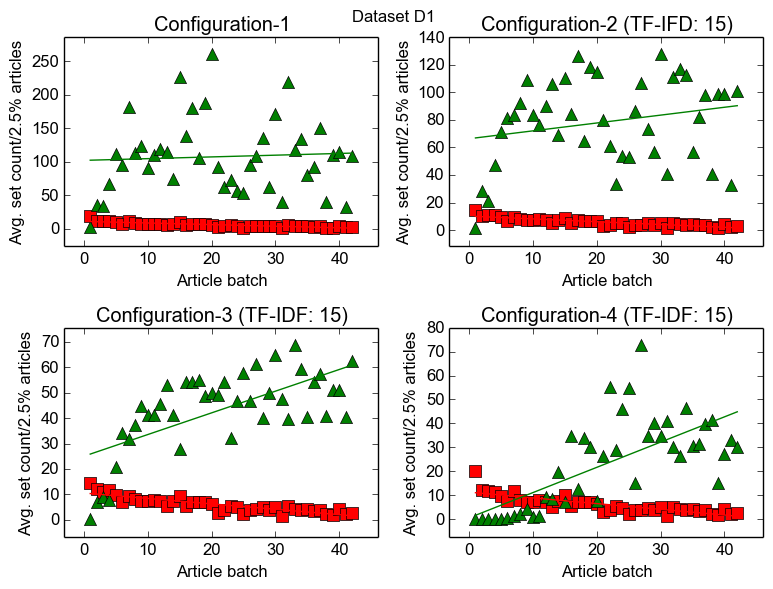
\includegraphics[scale=0.70]{images/D1-plot.png}
  \caption{Average number of new words and new pairs per batch of 2.5\% of all articles in dataset D1}
  \label{fig:setPlot1}
\end{figure}

\begin{figure}[h]
  \centering
  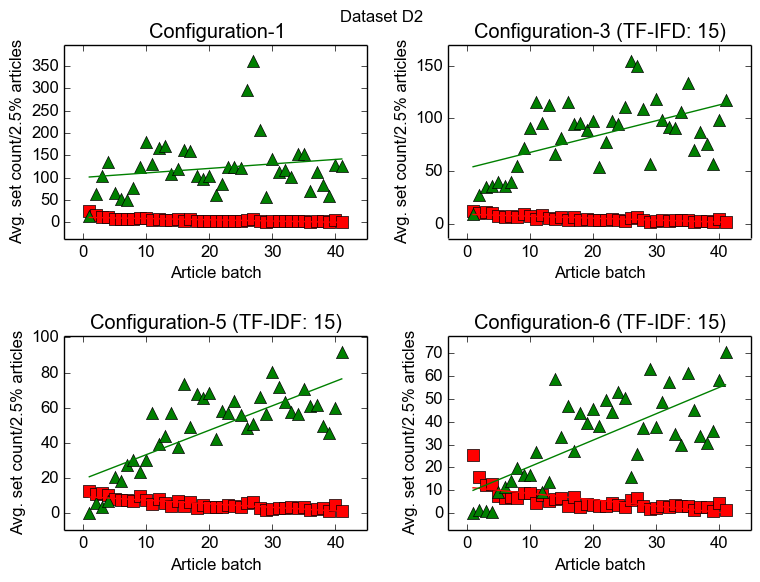
\includegraphics[scale=0.70]{images/D2-plot.png}
  \caption{Average number of new words and new pairs per batch of 2.5\% of all articles in dataset D2}
  \label{fig:setPlot2}
\end{figure}

\begin{figure}[h]
  \centering
  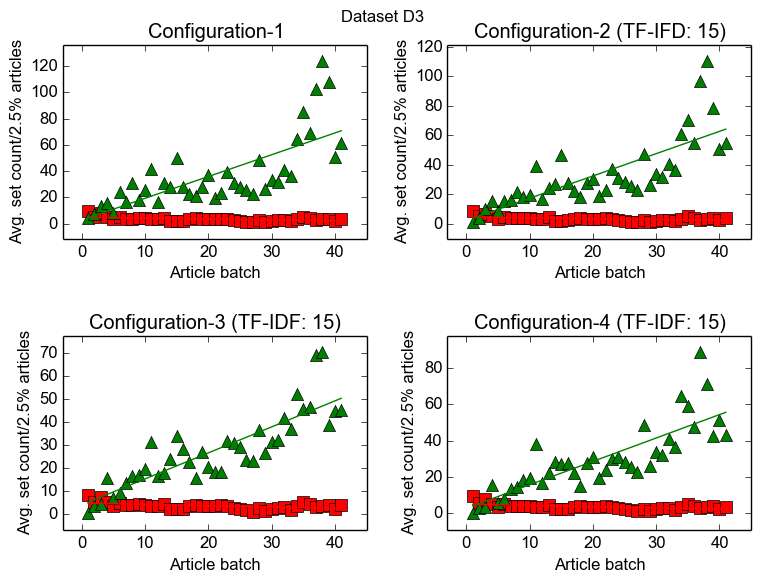
\includegraphics[scale=0.70]{images/D3-plot.png}
  \caption{Average number of new words and new pairs per batch of 2.5\% of all articles in dataset D3}
  \label{fig:setPlot3}
\end{figure}

\begin{figure}[h]
  \centering
  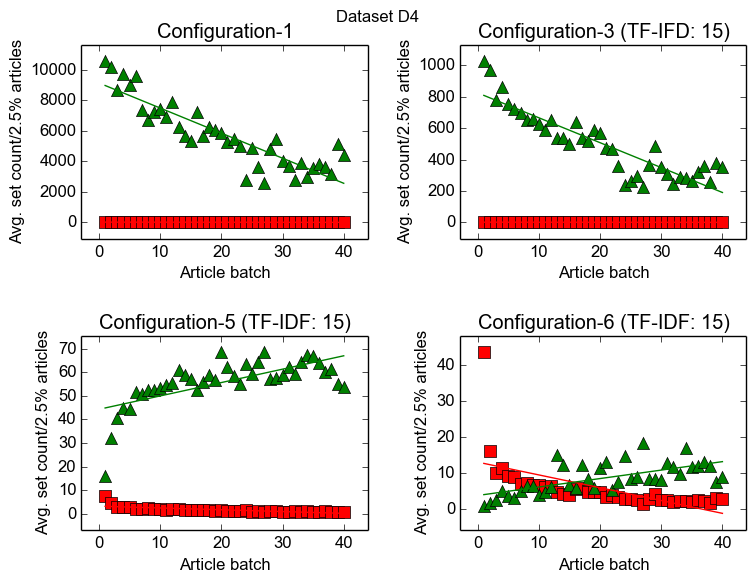
\includegraphics[scale=0.70]{images/D4-plot.png}
  \caption{Average number of new words and new pairs per batch of 2.5\% of all articles in dataset D4}
  \label{fig:setPlot4}
\end{figure}

\Crefrange{fig:setPlot1}{fig:setPlot4} show how the amount of minimal new sets of size less than 3 found in enumeration changes over time using different configurations. In all cases the amount of new words found decreases over time while the amount of new pairs found tends to increase over time.
